\documentclass[aps, pre, onecolumn, nofootinbib, notitlepage, groupedaddress, amsfonts, amssymb, amsmath, longbibliography, superscriptaddress]{revtex4-1}
\usepackage{tabularx}
\usepackage{graphicx}
\usepackage{hyperref}
\usepackage{xcolor}
\hypersetup{
    colorlinks,
    linkcolor={red!50!black},
    citecolor={blue!50!black},
    urlcolor={blue!80!black}
}
\usepackage{bm}
\usepackage{natbib}
\usepackage{longtable}
\LTcapwidth=0.87\textwidth

\newcommand{\Div}[1]{\ensuremath{\nabla\cdot\left( #1\right)}}
\newcommand{\DivU}{\ensuremath{\nabla\cdot\bm{u}}}
\newcommand{\angles}[1]{\ensuremath{\left\langle #1 \right\rangle}}
\newcommand{\KS}[1]{\ensuremath{D_{\text{KS}}(#1)}}
\newcommand{\KSstat}[1]{\ensuremath{\overline{D_\text{KS}(#1)}}}
\newcommand{\grad}{\ensuremath{\nabla}}
\newcommand{\RB}{Rayleigh-B\'{e}nard }
\newcommand{\Reff}{\ensuremath{\text{Re}_{\text{ff}}}}
\newcommand{\Peff}{\ensuremath{\text{Pe}_{\text{ff}}}}


\newcommand\mnras{{MNRAS}}%
\newcommand\apjl{{The Astrophysical Journal Letters}}%

\begin{document}
\author{Evan H. Anders}
\affiliation{Dept. Astrophysical \& Planetary Sciences, University of Colorado -- Boulder, Boulder, CO 80309, USA}
\affiliation{Laboratory for Atmospheric and Space Physics, Boulder, CO 80303, USA}
\author{Geoffrey M. Vasil}
\affiliation{University of Sydney School of Mathematics and Statistics, Sydney, NSW 2006, Australia}
\author{Benjamin P. Brown}
\affiliation{Dept. Astrophysical \& Planetary Sciences, University of Colorado -- Boulder, Boulder, CO 80309, USA}
\affiliation{Laboratory for Atmospheric and Space Physics, Boulder, CO 80303, USA}
\author{Lydia Korre}
\affiliation{Laboratory for Atmospheric and Space Physics, Boulder, CO 80303, USA}
\author{Jeffrey S. Oishi}
\affiliation{Department of Physics and Astronomy, Bates College, Lewiston, ME 04240, USA}

\title{Thermal relaxation is important in convective simulations: \\
on the time evolution of flows and how to avoid unnecessary thermal rundown}

\begin{abstract}
Astrophysical studies of convection often impose different thermal boundary conditions at the top and the bottom of the domain in an effort to more accurately reflect the natural system being modeled.
In this work, we study \RB convection (RBC) to show that the use of these mixed thermal boundary conditions imposes a long thermal rundown on convective systems which is not experienced by the more classical system where the temperature is fixed at the top and bottom of the domain.
We demonstrate that the mean behavior of an evolved simulation with mixed thermal boundaries corresponds to an equivalent simulation with fixed temperature boundaries at the top and bottom.
We show that the fast evolution of fixed-temperature simulations can be taken advantage of to rapidly relax simulations with mixed boundaries.
In the measurements presented here, we find that the asymmetries created by mixed boundaries do not importantly affect spatially averaged dynamics, but we do find that more extreme values of temperature can occur near a fixed flux boundary than a fixed temperature boundary.
We also demonstrate that these findings carry over to more complicated problems through a brief examination of rotating convection.
These results suggest that thermal relaxation occurs in two stages: (1) changes to the experimental energy reservoir and (2) changes to the stratification of the experiment.
Through the proper choice of boundary conditions or initial conditions, the first of these stages can be bypassed, and the second stage seems to be irrelevant for RBC.
\end{abstract}
\maketitle

%%%%%%%%%%%%
%%%%%%%%%%%
% INTRO
%%%%%%%%%%%
%%%%%%%%%%%%

\section{Introduction}
\label{sec:introduction}
Convection is a crucial heat transport mechanism in the atmospheres and interiors of stars and planets.
The nature of astrophysical convection is primarily studied through the use of numerical simulations which range from studies of the highly simplified Boussinesq approximation \cite{spiegel&veronis1960} to more complex ``dynamo simulations'' which include magnetism and atmospheric density stratification \cite{charbonneau2014, toomre2019}.
Regardless of the degree of apparent realism of the employed simulations, numerical convection is fundamentally driven by some combination of imposed boundary conditions and internal heating profiles \cite{goluskin2015}.
A common choice of thermal boundary conditions in astrophysical convection \cite{glatzmaier&gilman1982, hurlburt&all1986, cattaneo&all1990, featherstone&hindman2016a, korre&all2019, wood&brummell2018, kapyla&all2019} is to fix the flux at the bottom boundary and to fix the value of a thermodynamic quantity (e.g., temperature) at the top boundary.
In this work, we will examine the consequences of these ``mixed'' boundaries in the simplest possible model: \RB convection (RBC) under the Boussinesq approximation.
In this model, temperature is the only thermodynamic quantity and we use the term ``FT'' boundaries to refer to the choice of fixing the flux at the bottom and the temperature at the top of the simulation.

Despite FT boundary conditions being frequently used, we are unaware of any study which has aimed to understand the consequences of imposing FT boundaries compared to the most classic RBC setup where the temperature is fixed at the top and bottom (hereafter ``TT'' boundaries\footnote{Note, in ref.~\cite{goluskin2015}, our TT and FT are repsectively called RB1 and RB3.}).
It is generally assumed that FT boundaries should behave fundamentally similarly to a system in which the flux is fixed at both boundaries (hereafter ``fixedF'' boundaries), whose behavior is well-known \cite{otero&all2002, goluskin2015}.
FixedF and TT boundaries have been shown to produce the same scaling of heat transport as the convective is ddriven more strongly \cite{johnston&doering2009}, and it is natural to assume that FT should fall on the same scaling laws.
However, the choice of FT boundaries introduces complexities into the convective system which neither fixedF or TT boundaries are exposed to.
First, the evolved mean temperature of a simulation with FT boundaries differs from the initial mean temperature, and therefore the thermal reservoir of the convective system must evolve over time.
Second, FT boundary conditions are fundamentally asymmetric, and the degree to which these boundary conditions break the symmetry of the system is unclear.

In this paper, we investigate the time evolution and nature of asymmetries in \RB covection when FT boundary conditions are imposed.
We also compare the flows in evolved, thermally relaxed FT simulations to the flows in evolved TT simulations.
We find that the thermal evolution and relaxation of FT systems is very long compared to TT systems, where it is nearly instantaneous.
However, this long thermal evolution can be bypassed by using the results of TT simulations as initial conditions for FT simulations.
If a FT simulation is allowed to relax through its natural thermal rundown, these simulations perform a sweep through parameter space where the dynamical nature of the early flows are very different from those of the relaxed flows.
Our results also suggest that the choice of FT boundaries imposes some asymmetries on the convective flows, but that these asymmetries do not change the mean convective state when compared to TT siulations.
We present these findings as follows.
In section \ref{sec:simulations}, we describe our simulation setup and numerical methods.
In section \ref{sec:2d_results}, we first describe our findings with respect to the time evolution of FT systems, and then describe the asymmetries in these systems.
In section \ref{sec:rotating_results}, we show that these findings carry over to a more complex system: rotating \RB convection.
Finally, in section \ref{sec:discussion}, we summarize our findings and briefly describe the implications of this work for the field of astrophysical convection.

%%%%%%%%%%%%
%%%%%%%%%%%
% EXPERIMENT
%%%%%%%%%%%
%%%%%%%%%%%%

\section{Simulation Details}
\label{sec:simulations}
We study incompressible \RB convection under a freefall nondimensionalization as we have done previously \cite{anders&all2018}; for details of the nondimensionalization, we refer readers to that previous work.
In section \ref{sec:rotating_results} we study convection which includes the effects of vertical global rotation \cite{julien&all1996}, so here we include the Coriolis term in the momentum equation for generality.
The equations of motion are
\begin{align}
\Div{\bm{u}} &= 0
	\label{eqn:incompressible}
\\
\frac{\partial \bm{u}}{\partial t} + \left(\bm{\omega} + \frac{1}{\text{Ek }\Reff}\hat{z}\right)\times\bm{u} 
&= - \grad \varpi + T_1\hat{z} - \frac{1}{\Reff}\grad\times\bm{\omega},
	\label{eqn:bouss_momentum}
\\
\frac{\partial T_1}{\partial t}  + \bm{u}\cdot\grad T_1 + w \frac{\partial T_0}{\partial z} 
&= \frac{1}{\Peff}\grad^2 T_1,
	\label{eqn:bouss_energy}
\end{align}
where $\bm{u} = (u, v, w)$ is the velocity, $T = T_0(z) + T_1(x, y, z, t)$ is the temperature (where $T_0$ is the initial profile and $T_1$ is the fluctuations around that profile), $\varpi$ is the reduced kinematic pressure \cite{anders&all2018} which enforces the incompressible constraint, and $\bm{\omega} = \grad \times \bm{u}$ is the vorticity.
The dimensionless control parameters are the Rayleigh, Prandtl, and Ekman numbers,
\begin{equation}
\text{Ra} = \frac{g \alpha L_z^3 \Delta}{\nu\kappa} = \frac{(L_z\,v_{\text{ff}})^2}{\nu\kappa}, \qquad \text{Pr} = \frac{\nu}{\kappa}, \qquad \text{Ek} = \sqrt{\frac{\nu}{2\Omega L_z^2}},
\end{equation}
where $g$ is the gravity, $\alpha$ is the coefficient of thermal expansion, $L_z$ is the domain depth, $\nu$ and $\kappa$ are respectively the viscous and thermal diffusivity, and $\Omega$ is the global rotation frequency.
These parameters set the freefall Reynolds and Peclet numbers, $\Reff = \sqrt{\text{Ra}/\text{Pr}}$ and $\Peff = \text{Pr }\Reff$, and throughout this work we hold Pr = 1 so that $\Reff = \Peff$.
In standard RBC without rotation (section \ref{sec:2d_results}), we set Ek$\,= \infty$.
The extent of our numerical domain is $z = [-0.5, 0.5]$ vertically and $x, y = [-\Gamma/2, \Gamma/2]$, where $\Gamma$ is the aspect ratio.
The initial temperature profile, $T_0(z) = 0.5 - z$, is unstable and linearly decreases from a value of 1 to 0 across the domain. 
$\Delta$ is the dimensionless temperature jump across the domain; depending on our choice of boundary condition, $\Delta$ defines either a temperature or flux Rayleigh number,
\begin{equation}
\text{Ra}_{\Delta T} = \frac{g \alpha L_z^3 \Delta T_0}{\nu\kappa}, \qquad 
\text{Ra}_{\partial_z T} = \frac{g \alpha L_z^4 \partial_z T_0}{\nu\kappa}.
\end{equation}
We study both FT and TT thermal boundary conditions,
\begin{equation}
(\text{FT}): T_1 = 0 \text{ at $z$ = 0.5} \,\,\,\&\,\,\, \partial_z T_1 = 0 \text{ at $z$ = -0.5};\qquad\qquad
(\text{TT}): T_1 = 0 \text{ at $z$ = \{-0.5, 0.5\}}.
\end{equation}
In the case of FT boundaries, the temperature is nondimensionalized on the initial temperature gradient, $\Delta = L_z \partial_z T_0$, and the input Rayleigh number is a flux Rayleigh number, Ra$_{\partial_z T}$.
In the case of TT boundaries, the temperature is nondimensionalized on the initial temperature jump across the domain: $\Delta = \Delta T_0 =  T_0(z=0.5)-T_0(z=-0.5)$, and the input Rayleigh number is a temperature Rayleigh number, Ra$_{\Delta T}$.



Throughout the bulk of this work, we study two-dimensional (2D) convection where $\partial_y = v = 0$.
For comparison with the literature, we specify $\Gamma = 2$ and these simulations employ no-slip, impenetrable boundaries,
\begin{equation}
u = w = 0 \, \, \text{at}\,\,z = -0.5, 0.5.
\label{eqn:vel_bcs}
\end{equation}
The rotating cases in section \ref{sec:rotating_results} are three-dimensional (3D) tall, skinny boxes with $\Gamma = 10\lambda_c(\text{Ek})$, where $\lambda_c(\text{Ek})$ is the wavelength of convective onset at the specified value of Ek, as has been done by previous authors \cite{stellmach&all2014}. 
These rotating simulations employ stress-free, impenetrable boundaries,
\begin{equation}
\partial_z u = \partial_z v = w = 0 \, \, \text{at}\,\,z = -0.5, 0.5.
\label{eqn:vel_bcs}
\end{equation}

We utilize the Dedalus\footnote{\url{http://dedalus-project.org/}} pseudospectral framework \cite{burns&all2016, burns&all2019} to evolve Eqs.~(\ref{eqn:incompressible}-\ref{eqn:bouss_energy}) forward in time.
Our 2D simulations use an implicit-explicit (IMEX), third-order, four-stage Runge-Kutta timestepping scheme RK443; our 3D rotating simulations use the second-order, two-stage Runge-Kutta scheme RK222 \cite{ascher&all1997}. 
The code used to run simulations and to create the figures in this work are available publicly online in a repository of supplemental materials \cite{anders&all2020a_supp}.
Variables are time-evolved on a dealiased Chebyshev (vertical) and Fourier (horizontal, periodic) domain in which the physical grid dimensions are 3/2 the size of the coefficient grid.  
We fill $T_1$ with random white noise whose magnitude is $10^{-6}/\Peff$, and which is vertically tapered to zero at the boundaries.
We filter this noise spectrum in coefficient space, such that only the lower 25\% of the coefficients have power; this low-pass filter is used to avoid populating the highest wavenumbers with noise in order to improve the stability of our spectral timestepping methods.


%%%%%%%%%%%%%%%%%%%%%%%%%%%%%%%%%%%%
%%%%%%%%%%%%%%%%%%%%%%%%%%%%%%%%%%
% Ra & Nu arguments
%%%%%%%%%%%%%%%%%%%%%%%%%%%%%%%%%%
%%%%%%%%%%%%%%%%%%%%%%%%%%%%%%%%%%%%
\subsection{Nondimensional Output Quantities}
\label{sec:ra_nu_relations}
Throughout this work we will measure and report the evolved value of the Nusselt number.
We define and measure the Nusselt number instantaneously as
\begin{equation}
\text{Nu} \equiv \angles{\frac{w T - \Peff^{-1} \partial_z T}{-\Peff^{-1} \angles{\partial_z T}}}
= 1 + \Peff\frac{\angles{w T}}{-\Delta T},
\end{equation}
where $\angles{}$ represent a volume average ($\angles{A} \equiv \iint A\,dx\,dz / \Gamma$ in 2D and $\angles{A} \equiv \iiint A\,dx\,dy\,dz / \Gamma^2$ in 3D for some quantity $A$), and $\Delta T = \angles{\partial_z T}$ is the temperature difference between the top and bottom plate.
In the evolved, statistically stationary state, when TT boundaries are employed, $\text{Nu} = 1 + \Peff\angles{wT} = \text{(Evolved Flux)\Peff}$, and when FT boundaries and a flux nondimensionalization are employed, $\text{Nu} = (\Delta T)^{-1}$.
This suggests that the equilibrated state of a given convective solution is characterized by both a flux and temperature Rayleigh number whose relationship is
\begin{equation}
\text{Ra}_{\partial_z T} = \text{Ra}_{\Delta T} \text{Nu}.
\label{eqn:ra_relation}
\end{equation}
In other words, in addition to measuring the efficiency of convective heat transport, the Nusselt number is also the unit of conversion between a temperature and a flux nondimensionalization in the evolved state.

Some additional quantities of interest will be reported throughout this paper.
We will measure the evolved Peclet number of the convective flows in all sections, and in section \ref{sec:rotating_results} we will also report the value of the Rossby number.
We measure these nondimensional quantities instantaneously as
\begin{equation}
\text{Pe} = \angles{|\bm{u}|}\Peff,\qquad \text{Ro} = \angles{|\bm{\omega}|}\text{Ek }\Reff,
\end{equation}
where $|\bm{A}|$ represents the magnitude of the vector $\bm{A}$.





%%%%%%%%%%%%
%%%%%%%%%%%
% RESULTS
%%%%%%%%%%%
%%%%%%%%%%%%
\section{Results}
\label{sec:2d_results}

\subsection{Time Evolution}

\begin{figure}
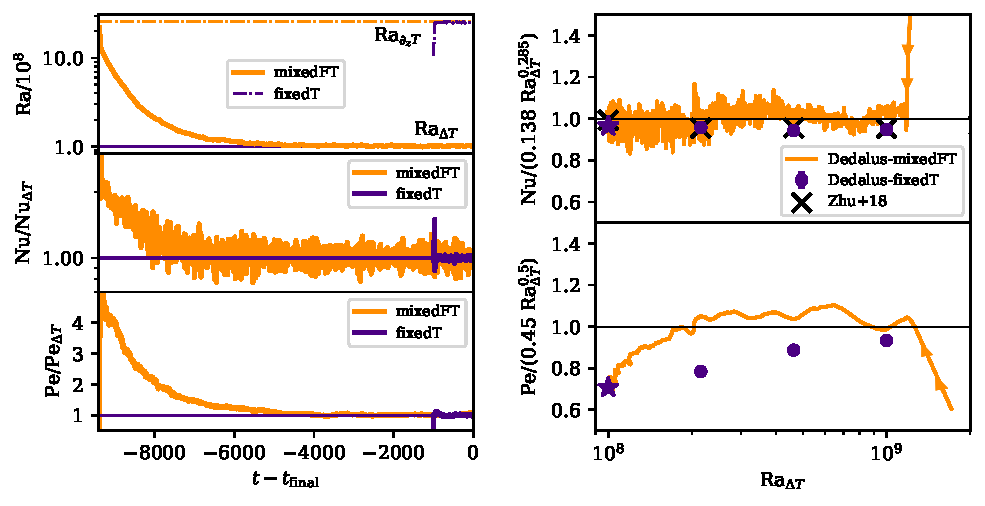
\includegraphics[width=\textwidth]{./figs/rbc_scalar_comparisons.pdf}
\caption{ 
	(left three panels) Time traces of rolling averages over 50 freefall times of a FT (orange) and a TT (purple) simulation.
	(top left panel) The Rayleigh number, normalized by the input Ra$_{\Delta T}$ = $10^8$ value of the TT simulation.
	(middle and bottom left panels) The evolution of Nu and Pe is shown, and is normalized by the mean value measured over the last 500 freefall times of the TT simulation (reported in appendix \ref{app:table}).
	(right two panels) Compensated parameter space plots of Nu (upper) and Pe (lower) vs. Ra$_{\Delta T}$.
	The Nu vs Ra plot is compensated by $(0.138 \text{Ra}_{\Delta T}^{0.285})$, which was the best-fit reported by ref.~\cite{johnston&doering2009}.
	The Re vs Ra plot is compensated by a Ra$_{\Delta T}^{1/2}$ law, which is the anticipated scaling of the Peclet number \cite{ahlers&all2009}.
	The time evolution of the FT case is shown as an orange trace with the arrows showing the sense of time.
	Purple circles show our measured values of Nu in TT simulations (reported in appendix \ref{app:table}); error bars show the standard deviation of the sample mean and are smaller than the marker in all cases.
	The orange star in each plot corresponds to the TT case whose time evolution is shown on the left.
	Black crosses show comparison TT simulations as reported by ref.~\ref{zhu&all2018}.
\label{fig:rbc_scalar_comparisons} }
\end{figure}

In Fig.~\ref{fig:rbc_scalar_comparisons}, we describe the evolution of a FT simulation which is characterized by Ra$_{\partial_z T}$ = 2.61$\,\times 10^9$.
The left panels of Fig.~\ref{fig:rbc_scalar_comparisons} compare this simulation to a TT case with Ra$_{\Delta T} = 10^8$.
The FT case is displayed in orange, and the TT case is displayed in purple; the x-axis of the left panels shows simulation time, in freefall units, with the time of the simulation's end subtracted from it (such that $x = 0$ corresponds to the end of the simulation).
In the top-left panel, we compare the evolution of the Rayleigh number of these simulations: temperature Rayleigh numbers, Ra$_{\Delta T}$ are displayed as solid lines, and flux Rayleigh numbers, Ra$_{\partial_z T}$ are shown as dash-dot lines.
The value of Ra$_{\Delta T}$ takes thousands of time units to reach its final value for the FT simulation, and this final value corresponds to the input value of the equivalent TT case.
On the other hand, the value of Ra$_{\partial_z T}$ for the TT case nearly instantaneously reaches its final value, which corresponds to the input value for the FT simulation.
This discrepancy in evolution timescales, where TT simulations evolve quickly and FT simulations evolve slowly, is also seen in the equilibration of the Nusselt number (middle panel) and Peclet number (bottom panel).
All time traces displayed are rolling averages over 50 freefall times, in order to reduce the variance of the plotted quantities.

In the right panels of Fig.~\ref{fig:rbc_scalar_comparisons}, we plot compensated scaling plots of Nu and Pe vs Ra$_{\Delta T}$.
Over the course of its thermal relaxation, the FT case performs a sweep through Ra$_{\Delta T}$ parameter space.
During this parameter space sweep, the FT simulation seems to trace out the expected scaling law of Nu vs.~Ra displayed by TT simulations and which has been reported by previous authors.
However, we find that the value of Pe measured in the FT simulation through its relaxation  is larger than the value of the Peclet number in comparison TT simulations until it converges to its final state.
These traces through parameter space demonstrate the importance of waiting until a FT simulation has reached its equilibrated state.
During the rundown, the dynamics in FT simulations are constantly evolving, and also they display more vigorous convection than in equivalent converged states, suggesting that the dynamics do not immediately ``forget'' the higher-Ra$_{\Delta T}$ state that they were previously in during the parameter space sweep.
Both of these effects make interpretation of their results difficult until the final, equilibrated state.

\begin{figure}
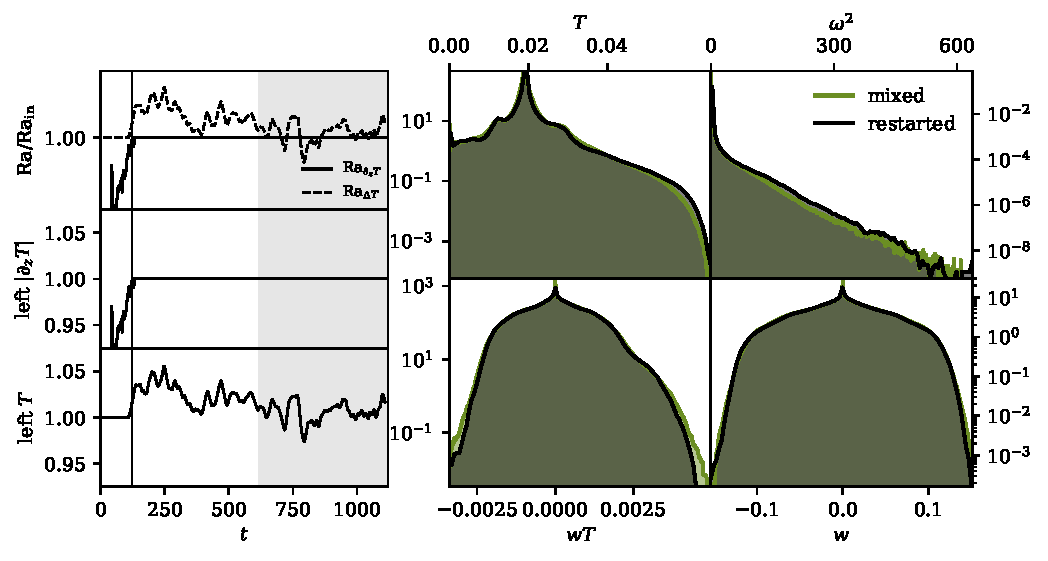
\includegraphics[width=\textwidth]{./figs/rbc_restart_description.pdf}
\caption{ 
	(left three panels) Time traces of rolling averages over 25 freefall times of a simulation which starts with TT boundary conditions and then is switched to FT boundary conditions.
	The time at which we switch from TT to FT boundaries is noted by the vertical black line.
	(top left panel) The Rayleigh number's evolution over time is shown; Ra$_{\partial_z T}/(2.61\times 10^9)$ is shown as a dashed-dot line, while Ra$_{\Delta T}/10^8$ is shown as a solid line.
	The mean value of the bottom boundary's temperature gradient (middle panel) and temperature (bottom panel) are consistently nondimensionalized and displayed, showing the change in the enforced boundary condition.
	In the TT initial state, the temperature is held constant at a value of 1 and the temperature derivative fluctuates around a value of $\angles{\text{Nu}}$.
	In the FT final state, the temperature derivative is held constant at a value of -1 and the temperature value fluctuates around a value of $\angles{\text{Nu}}^{-1}$.
	(right four panels) Probability distribution functions of dynamics at all spatial points in the domain sampled once each freefall time for a total of 500 freefall times are shown.
	We display the temperature field (upper left), enstrophy (upper right), nonlinear convective enthalpy flux (bottom left), and vertical velocity (bottom right).
	In each plot, we compare the PDF of the FT case which thermally relaxed (in Fig.~\ref{fig:rbc_scalar_comparisons}) to the PDF of the ``t-to-m'' (TT-to-FT) case which is drawn from dynamics in the grey shaded region displayed in the left three panels here.
\label{fig:rbc_restart_description} }
\end{figure}

The equivalence of the evolved values of Ra, Nu, and Pe in Fig.~\ref{fig:rbc_scalar_comparisons} between the FT and TT simulations suggests that, in a volume-averaged sense, there is a comparable TT experiment for each FT experiment.
It should therefore be possible to take advantage of the fast evolution of TT simulations to achieve rapidly equilibrated FT simulations, which would save a great deal of computing time in solving FT simulations.
The rundown in FT simulations is very costly for two reasons: the turbulent dynamics at the large initial Ra$_{\Delta T}$ require more spectral modes to resolve than the equilibrated state and thousands of freefall times must pass during relaxation.
For example, for the cases displayed in Fig.~\ref{fig:rbc_scalar_comparisons}, the first thousand freefall time units took $1.43\times10^6$ iterations, or roughly $3.3 \times 10^4$ cpu-hours for the FT simulation, but only  $8.4\times10^5$ iterations, or roughly $5.4\times 10^3$ cpu-hours for the TT simulation.
After these thousand freefall time units, the TT simulation has spent hundreds of freefall times in a statistically stationary relaxed state, whereas the FT system continues to evolve towards its equilibrium state for an additional few thousands of time units.
Even at these modest Rayleigh numbers (Ra$_{\Delta T} = 10^8$), the cost of equilibration of a FT simulation is therefore more than an order of magnitude larger than a TT simulation.

We now describe a procedure which takes advantage of the fast evolution of TT simulations to achieve equilibrated FT simulations.
In short, the full evolved flow fields in the TT simulation are properly re-nondimensionalized and used as initial conditions for a FT simulation.
To achieve this, we perform these steps:
\begin{enumerate}
\item Run a TT simulation to its statistically stationary state ($\sim100+$ time units). 
Measure $\angles{\text{Nu}}$ in that state.
\item Re-nondimensionalize from $\Delta = \Delta T \rightarrow \partial_z T$, and from Ra$_{\Delta T}\rightarrow$Ra$_{\partial_z T}$, as in Eqn.~\ref{eqn:ra_relation}.
In our freefall nondimensionalization, this means setting the velocities in the FT simulation to $\bm{u}_{\text{FT}} = \bm{u}_{\text{TT}} / \sqrt{\angles{\text{Nu}}}$, and setting the temperature field to $T_{\text{FT}} = T_{\text{TT}} / \angles{\text{Nu}}$.
\item Restart the simulation with FT boundaries and continue timestepping.
\end{enumerate}
In the left panels of Fig.~\ref{fig:rbc_restart_description}, we show time traces of a simulation in which we employ this procedure.
We initialize a TT simulation at Ra$_{\Delta T} = 10^8$, which has been reported to have $\text{Nu} \approx 26.1$ \cite{zhu&all2018}.
Roughly one hundred freefall times after the convective transient, we restart this simulation using FT boundaries according to our above procedure with an input Ra$_{\partial_z T} = 2.61 \times 10^9$, and we run this simulation for a further thousand time units.
We note that this is the same Ra$_{\partial_z T}$ as the FT case presented in Fig.~\ref{fig:rbc_scalar_comparisons}.
In the left panels, we show the temporal behavior of the Rayleigh numbers (top panel), and the flux (middle panel) and temperature (bottom panel) at the bottom boundary of the simulation.
The change from TT to FT boundaries is shown as a vertical line.
Unlike in the FT case displayed in Fig.~\ref{fig:rbc_scalar_comparisons}, there is no long thermal rundown in the FT state, due to the rapid relaxation achieved during the TT portion of the simulation.

While these time traces show that this procedure bypasses the long thermal rundown on display in Fig.~\ref{fig:rbc_scalar_comparisons}, this does not prove that the dynamics in the final state faithfully reproduce those achieved by a thermal rundown.
We now compare probability distribution functions (PDFs) of various quantities in our restarted FT simulation to the FT simulation that stepped through a long rundown.
For the last 500 freefall times of each simulation (e.g., the grey shaded region in Fig.~\ref{fig:rbc_restart_description}), we sample the full flow field once each freefall time.
We interpolate the (unevenly spaced) vertical chebyshev gridpoints onto an evenly spaced grid before histogramming flow values using 500 bins.
In the right four panels of Fig.~\ref{fig:rbc_restart_description}, we display PDFs of the temperature field (upper left), enstrophy (upper right), convective flux (lower left), and vertical velocity (lower right).
In Table~\ref{table:pdf_values}, we display the first four moments of each of these distributions,
\begin{equation}
\begin{split}
&\mu(A) \equiv \sum_{i} A_i\,P(A_i)\,\Delta A,\qquad\qquad\qquad\qquad\qquad\qquad\,\,
\sigma(A) \equiv \sqrt{\sum_{i}[A_i-\mu(A)]^2 P(A_i) \Delta A},\\
&\text{Skewness}(A) \equiv \frac{1}{\sigma(A)^3}\sum_i [A_i-\mu(A)]^3 P(A_i) \Delta A,\qquad
\text{Kurtosis}(A) \equiv \frac{1}{\sigma(A)^4}\sum_i [A_i-\mu(A)]^4 P(A_i) \Delta A,
\end{split}
\label{eqn:pdf_moments}
\end{equation}
where $A$ is the quantity, $P(A)$ is the PDF of quantity $A$, $\mu$ is the mean, $\sigma$ is the standard deviation, $\Delta A$ is the spacing between the PDF bins, and $i$ is the index of the bin..
Visually the PDFs of dynamics in a FT and a restarted TT-to-FT simulation are essentially identical.
In all cases except for the enstrophy, the four moments of the PDFs between the two runs are also very similar.
These simulations have no-slip boundaries, so the enstrophy is concentrated near the plume impacting sites within the boundary layers.
The small differences between the enstrophy PDFs perhaps points to slightly different plume morphologies being sampled during the 500 freefall time units in the two runs, but the similarities between the two cases in other important quantities (specfically in nonlinear transport) lead us to believe that this difference is unimportant.

\begin{table}[t!]
\caption{ 
	The first four moments, as defined in Eqn.~\ref{eqn:pdf_moments}, of each of the PDFs shown in Fig.~\ref{fig:rbc_restart_description} are displayed below.
}
\setlength{\tabcolsep}{12pt}
\label{table:pdf_values}
\begin{center}
\begin{tabularx}{\textwidth}{c c c c c c}
\hline																	
Quantity &	Case	&	$\mu$	&	$\sigma$	&	Skewness	&	Kurtosis \\
%\hline \hline \multicolumn{6}{c}{\vspace{-0.2cm}}\\
%\multicolumn{6}{c}{\vspace{0.1cm}2D Runs} \\
\hline
$T$				&	FT		&		$1.9 \times 10^{-2}$	&	$4.3 \times 10^{-3}$	&	1.1		&	15 \\
				&	FT,r	&		$1.9 \times 10^{-2}$	&	$4.3 \times 10^{-3}$	&	1.3		&	18 \\
\hline
$\omega^2$		&	FT		&		$1.3$					&	$6.4$					&	19		&	$5.2 \times 10^2$ \\
				&	FT,r	&		$3.9$					&	$7.4$					&	18		&	$4.5 \times 10^2$ \\
\hline
$wT$			&	FT		&		$1.9 \times 10^{-5}$	&	$9.4 \times 10^{-4}$	&	0.16	&	$3.1$ \\
				&	FT,r	&		$1.9 \times 10^{-5}$	&	$9.3 \times 10^{-4}$	&	0.16	&	$3.1$ \\
\hline
$w$				&	FT		&		$7.9 \times 10^{-7}$	&	$4.9 \times 10^{-2}$	&	0.016	&	$2.7$ \\
				&	FT,r	&		$-5.2 \times 10^{-6}$	&	$4.8 \times 10^{-2}$	&	0.0066	&	$2.8$ \\
\hline																	
\end{tabularx}
\end{center}
\end{table}

We note briefly that this mechanism that we describe here is not the only mechanism for accelerating the thermal relaxation of a FT simulation.
We discuss other mechanisms, and explore one in detail, in our previous work \cite{anders&all2018}.
We note however that the TT-to-FT setup described here is likely the least complicated mechanism for achieving rapid relaxation in a simplified \RB convection setup that we are aware of.
The successful degree with which this mechanism reproduces the evolved dynamics suggests that thermal relaxation occurs in two parts:
\begin{enumerate}
\item Changes to the simulation energy reservoir, and
\item Restratification of the experiment.
\end{enumerate}
The rapid evolution of TT runs, whose energy reservoir does not change between the initial and final state, suggests that experimental restratification occurs rapidly in RBC. 
The long rundown of FT experiments on display in Fig.~\ref{fig:rbc_scalar_comparisons} is entirely due to the energy reservoir (the mean temperature) drifting over time.
Put differently, the classic \RB setup for $T_0(z)$ is a bad choice of initial conditions for FT boundaries, and our procedure uses TT dynamics to choose a more ideal set of initial conditions.

\subsection{Asymmetries induced by mixed boundaries}
\label{sec:asymmetries}
Now that we have verified a mechanism for rapidly and self-consistently achieving thermally equilibrated FT simulations, we study highly turbulent convection with FT boundaries in an effort to understand the nature of asymmetries introduced to the problem by these boundary conditions.
[NOTE: in the version of the paper that will be submitted, we will study Ra$_{\Delta T} = 10^{10}$ / Ra$_{\partial_z T} \sim 10^{12}$. These simulations are almost done running on Pleiades, so for now we'll carry on with the same values as in the previous section.]

\begin{figure}
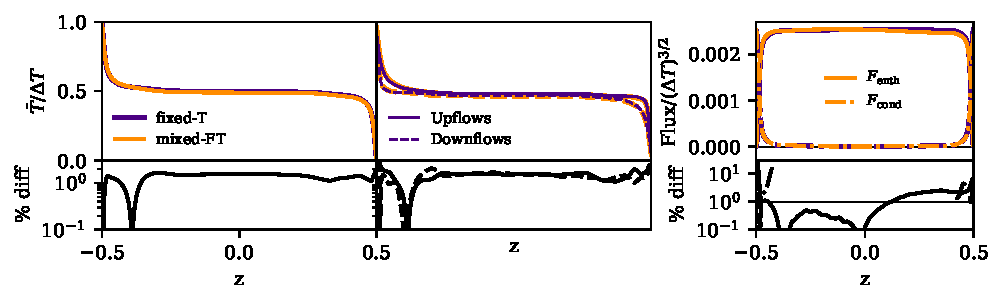
\includegraphics[width=\textwidth]{./figs/rbc_1D_profiles.pdf}
\caption{ 
	(upper left) The horizontally- and time-averaged temperature profile is shown for a FT (green) and TT (orange) simulation.
	(upper middle) The horizontally- and time-averaged temperature profile is shown for upflow regions (solid lines) and downflow regions (dashed lines) respectively.
	(upper right) The horizontally- and time-averaged fluxes in the system are shown.
	(bottom panels) The percentage difference between the corresponding quantities in the top panels are displayed, and in most cases measurements agree to within a few percent through the full depth of the domain.
\label{fig:rbc_1D_profiles} }
\end{figure}

In Fig.~\ref{fig:rbc_1D_profiles}, we compare the horizontally averaged, vertical profiles of our TT and FT cases.
In the upper left panel, we show the mean temperature profiles achieved in the evolved state of both simulations.
Throughout the full depth, these profiles differ by less than 2\%, as shown in the lower left panel.
In the upper middle panel, we show the mean temperature profile in downflow areas compared to the mean temperature profile achieved in upflow areas.
Surprisingly, despite symmetrical boundary conditions in TT simulations and asymmetrical boundary conditions in FT cases, we on average find precisely the same asymmetries in upflows/downflows for both sets of boundary conditions.
In general, we find that the boundary layer in upflows is more gradual in hot plumes, and the same is true for downflows and cold plumes.
Once again, these profiles agree to within $< 2\%$.

In the upper right panel of Fig.~\ref{fig:rbc_1D_profiles}, we plot the system fluxes for both cases, which also show good agreement between FT and TT.
Throughout the bulk of the domain, the convective enthalpy fluxes agree to within a few \% or less (solid line in bottom right panel).
Due to the conductive fluxes approaching zero in the interior, we cannot measure a \% difference for this flux in the bulk, but we find that it is again within a few percent in the boundary layers.
[NOTE: I need to figure out how to quantify the flux agreement better. Ideas?]

\begin{figure}
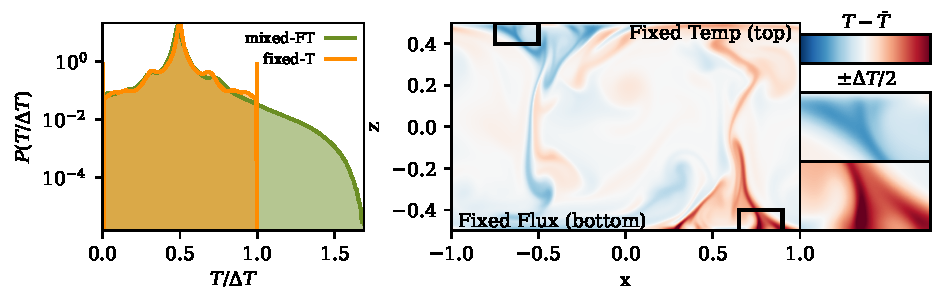
\includegraphics[width=\textwidth]{./figs/rbc_dynamics_asymmetries.pdf}
\caption{ 
	(left panel) PDFs of temperature measurements of a FT (orange) and TT (purple) case are displayed.
	The right tail of the distribution (near the cold fixed-flux boundary for the FT case) shows that fixed flux boundaries achieve more extreme temperature events than fixed temperature boundaries.
	(middle panel) A snapshot of the temperature anomaly in a FT simulation.
	The black outline boxes around the roots of the plumes are expanded in the bottom right panels.
	Near the top (fixed temperature) boundary, the temperature anomaly at the root of the plume vanishes near the boundary, but this does not happen near the bottom (fixed flux) boundary, allowing for more extreme instantaneous values.
\label{fig:rbc_dynamics_asymmetries} }
\end{figure}

In Fig.~\ref{fig:rbc_dynamics_asymmetries}, we examine the dynamical nature of the asymmetries which FT boundaries introduce into the simulation.
In the left panel, we plot PDFs of the temperature fields in comparable TT and FT simulations.
These PDFs agree remarkably well for cold temperatures (near the shared TT boundary) and through the mean, but diverge in the tail of the PDF for hot temperatures (where the boundary conditions differ).
Interestingly, there are no temperature fluctuations which exceed the specified boundary values in the convective domain for TT simulations.
However, the FT PDF has a much longer tail and achieves regions which are 50\% hotter than the average bottom boundary value.
In order to understand how this is possible, we examine a snapshot of the full temperature field.
In the middle panel, we plot the temperature anomaly, or the temperature field with the mean vertical profile subtracted from it.
We have outlined a portion of a cold plume near the upper (fixed-temperature) boundary and a portion of a hot plume near the lower (fixed-flux) boundary, and these regions are magnified in the rightmost panels.
The TT upper boundary suppresses temperature anomaly at the upper boundary and regulates the temperature minima which can be achieved.
The fixed-flux lower boundary does no such suppression and allows for extreme temperature values to be achieved in the plume-launching area, thus allowing for the asymmetry in the tails of the temperature PDF.

We note briefly that these asymmetries do not seem to affect mean or volume-averaged quantities in these simulations appreciably (see the agreement between FT and TT in Figs.~\ref{fig:rbc_scalar_comparisons}\&\ref{fig:rbc_1D_profiles}).
However, the fact that fixed-flux boundaries produce a wider temperature distribution with more extreme values may be important in some astrophysical studies.
We explore this further in the discussion in section \ref{sec:discussion}.





\section{Rotating \RB Convection}
\label{sec:rotating_results}
\begin{figure}
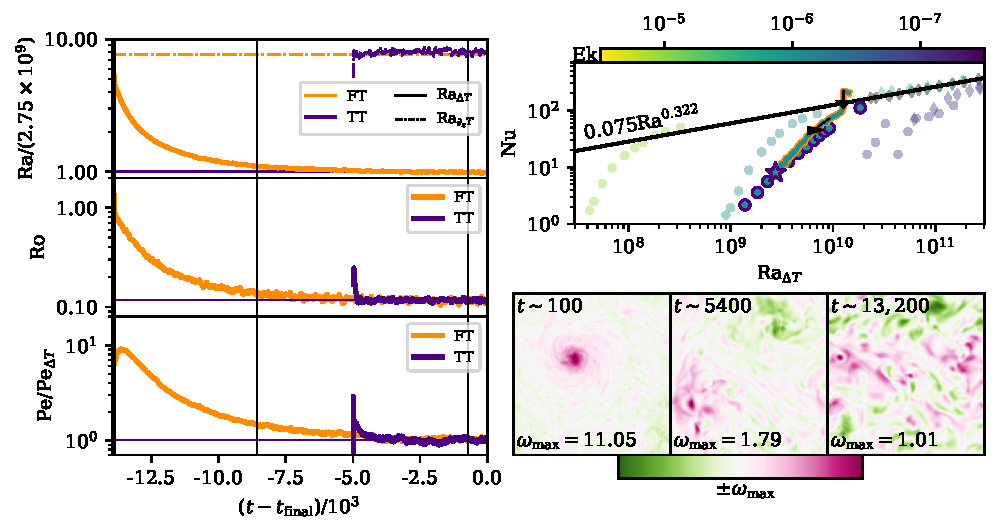
\includegraphics[width=\textwidth]{./figs/rotating_panels.pdf}
\caption{ 
	(left three panels) Time traces of rolling averages over 50 freefall times of a rotating FT simulation (green) and a TT (orange) simulation.
	(top left panel) The Rayleigh number, normalized by the input Ra$_{\Delta T}$ = 2.75$\,\times 10^9$ of the TT simulation.
	(middle left panel) The Rossby number evolution of both simulation; the bulk flow of the FT simulation transitions from a marginally rotationally constrained state to a heavily constrained state, while the TT simulation is in this latter state through its full evolution.
	(bottom left panel) The Peclet number evolution of the simulations is shown, normalized by the mean value measured over the last 500 freefall times of the TT simulation.
	(right upper panel) Parameter space plots of Nusselt vs. Ra$_{\Delta T}$.
	Circlular and diamond data points are respectively simulations and experimental data points from \cite{cheng&all2015}.
	The color of the data points signifies the Ekman number of the points, and black points are nonrotating.
	Data from our FT experiment are shown as a thick green trace, and the TT experiment's average is shown as a large orange star.
	(Bottom right panels) Snapshots of the vertically integrated z-component of the vorticity from the FT simulation.
	At early times (left panel), a powerful large scale vortex with positive vorticity develops.
	This vortex slowly decays and becomes a vortex pair (middle panel), as seen in \cite{stellmach&all2014}.
	In the converged state, we see oscillatory behavior between this vortex pair behavior and jets (right panel).
	The TT case exhibits the oscillatory behavior between vortex pairs and jets throughout its whole evolution.
	The three vertical black lines in the left panels signify the times at which this snapshots are taken.
\label{fig:rotating_panels} }
\end{figure}



We now extend our study of 2D RBC to a more complicated experiment.
Here, we examine 3D rotating RBC with an Ekman number of $10^{-6}$.
We study a TT case whose supercriticality is $\sim 3$ with Ra$_{\Delta T} = 2.75\times 10^9$, and a corresponding FT case with $\text{Ra}_{\partial_z T} = 2.1 \times 10^{10}$.
Both simulations have an aspect ratio $\Gamma = 0.481$, which is roughly ten times larger than the critical wavelength of TT convection at Ek = $10^{-6}$.
These simulations employ stress free boundary conditions which allow for the generation of mean flows such as large scale vortices \cite{couston&all2019}.

In the left three panels of Fig.~\ref{fig:rotating_panels}, we compare the time evolution of the FT and TT cases.
The top left panel shows the evolution of Ra$_{\partial_z T}$ and Ra$_{\Delta T}$.
Even in the presence of strong rotation, the TT case's fluxes immediately equilibrate, but the FT case takes thousands of freefall times to achieve thermal relaxation.
In the middle left panel, we show the evolution of the Rossby number.
While the evolved states of both simulations exhibit rotationally constrained dynamics with Ro $\,\sim 0.1$, the initial state of the FT simulation is only weakly rotationally constrained (Ro $\,\sim 1$).
The degree of rotational constraint felt by the flows decreases slowly toward its final state over thousands of freefall times.
In the bottom left panel, we display the evolution of the Peclet number over time.
Somewhat surprisingly, the peak value of Pe is found not during the convective transient but rather a few hundreds of freefall times later.
After achieving this peak value, the mean Pe monotonically decreases toward its final state.
We suspect that the initially large value of Ra$_{\Delta T}$ in the FT case drives high velocity flow associated with a developed large scale vortex (LSV).
As Ra$_{\Delta T}$ and convective driving decrease over time, the driving of the kinetic energy in this LSV eventually reaches an equilibrium value before decreasing, leading to the ``bump'' in the Pe trace.

In the upper right panel of Fig.~\ref{fig:rotating_panels}, we plot the evolution of Nu(t) vs.~Ra(t) for our FT case (thick orange line with teal interior) and the evolved value of Nu in the TT case (teal star with purple outline).
We have additionally plotted data from numerical simulations (circles) and experiments (diamonds) as reported in the appendix tables of ref.~\cite{cheng&all2015}.
The overplotted line is the best-fit line for values of Ra $\geq 10^{10}$ from ref.~\cite{cheng&all2015}.
We note that these comparison values are in cylindrical domains with Pr=7, whereas we are in Cartesian geometry with Pr=1, so some differences are expected.
As has been seen previously, the evolution of Nu vs.~Ra in the rotationally constrained regime is very steep compared to the nonrotating RBC cases in Fig.~\ref{fig:rbc_scalar_comparisons}.
The evolution of Nu(t) vs.~Ra(t) in the FT simulation seems to trace out the TT trend well, once again [NOTE: crap, I probably need some more TT comparisons. Bummer. They're fairly cheap, I'll sub them.].

In the bottom right panels of Fig.~\ref{fig:rotating_panels}, we examine the evolution of dominant flow structures over the course of thermal relaxation.
Shown is the vertically integrated vertical component of the vorticity.
As shown in the left panel, a dominant LSV which is aligned with the global rotation forms at early times.
Over thousands of freefall times, this LSV evolves into a long-lived vortex pair, displayed in the middle panel.
Finally, in the evolved state, this vortex pair solution begins to oscillate with domain-wide jets, such as those displayed in the right panel.
We find that the the TT solution shows this oscillatory behavior between vortex pairs and jets immediately and throughout the full 5000 frefall timescales of evolution that we simulated.

We note briefly that the transition from the unconstrained to rotationally constrained regime may be one area where the time evolution of FT simulations could be useful.
The scaling of Nu vs Ra in the rotationally constrained regime is more complex than in unrotational convection due to first order dominance of geostrophy \citep{julien&all2012, plumley&julien2019}.
A single FT simulation can trace through a large portion of this rotationally constrained parameter space, as shown in the upper right panel of Fig.~\ref{fig:rotating_panels}, so this approach may be one way to cleverly fill in this parameter space.
However, it is probable that the best course of action is simply to run a large suite of TT simulations that cover the same track for two reasons:
\begin{enumerate}
\item The long thermal rundown has some short-lived memory of the higher-Ra$_{\Delta T}$ state that it was recently in.
This is seen both in the post-transient bump of Pe in the bottom left panel of Fig.~\ref{fig:rotating_panels}, and also was found from a practical computing standpoint.
In order to reduce the computational cost of this FT simulation, we reduced the vertical resolution from $512\times384^2$ to $256\times384^2$ (after about 100 freefall times) and then later to $128\times384^2$ (after about $3.3 \times 10^3$ freefall times).
At each of these times, we found that lowering the \emph{horizontal} coefficient resolution of the simulation did not reproduced the simulation solution with fidelity.
For comparison, the TT simulation whose dynamics are identical to the evolved FT simulation was well resolved at a coefficient resolution of $128^3$.
This suggests that small scale turbulent velocity structure injected by the vigorous transient is long lived throughout the thermal evolution of the simulation.
\item The cost of running a turbulent FT simulation, compared to running its comparison TT simulation, is astounding.
The FT case ran for roughly $1.4 \times 10^4$ freefall time units total, and the number of iterations achieved per cpu-hour was $\sim$0.733 at $512\times384^2$, $\sim$2.03 at $256\times384^2$, and $\sim$6.79 at $128\times384^2$.
The simulation stepped through $1.59 \times 10^5$, $2.22 \times 10^6$, and $3.30 \times 10^6$ iterations at these resolutions, respectively, for a combined total of 2.32 million cpu-hours.
For comparison, the TT simulation ran for $5 \times 10^3$ freefall units at $128^3$, took 56.4 iterations per cpu-hour, and ran for $1.46 \times 10^6$ iterations, for $\sim 2.6 \times 10^4$ cpu-hours.
In other words, the computational cost of the FT simulation was \emph{two orders of magnitude} larger than its comparison TT case.
\end{enumerate}





%%%%%%%%%%%%
%%%%%%%%%%%
% CONCLUSION
%%%%%%%%%%%
%%%%%%%%%%%%

\section{Conclusions \& Discussion}
\label{sec:discussion}
In summary, we find that FT experiments experience a long thermal relaxation which is not experienced by TT simulations.
Here we have studied the time evolution of \RB convection under two different formulations of the thermal boundary conditions: ``FT'' boundaries, where the flux is fixed at the bottom and temperature is fixed at the top, and ``TT'' boundaries, where temperature is fixed at the top and bottom.
Through studying this relaxation and the relaxed states of both simulations, we come to the following conclusions:
\begin{enumerate}
\item Thermal relaxation in RBC has two components: (a) changes in the energy reservoir and (b) changes in the stratification.
We find that the long relaxation of FT simulations is due to changes in the energy reservoir; this reservoir is roughly constant in TT simulations due to the lack of evolution of the average domain temperature.
On the other hand, RBC seems to restratify itself nearly instantaneously, as suggested by the rapid equilibration of our TT simulations.
\item The thermal relaxation process of a FT simulation essentially performs a sweep through Ra$_{\Delta T}$ parameter space.
We find that the heat transport (the Nusselt number) follows classical scaling laws through this parameter space sweep, but does so in the presence of increased turbulent velocities (quantified by the Reynolds number).
\item Despite minor asymmetries in the instantaneously measured flows of FT simulations, we find no difference between the mean state of these simulations and the more classic TT simulations.
\item Great computational expense achieving thermal relaxation in a FT simulation can be avoided by using the evolved state of a TT simulation as a ``better'' set of initial conditions for a FT simulation.
In other words, the proper choice of initial conditions can ensure that the initial and evolved energy reservoirs are not vastly different.
\item If dynamical measurements are taken during the thermal relaxation of a FT simulation, they may be misleading.
Dynamics during the relaxation are in a more turbulent state than in the evolved state, and can even feel different flow balances in the equation of motion (as quantified by e.g., the Rossby number).
\end{enumerate}

[NOTE: This is basically wild speculation and flailing. I need to get refs in here, maybe rearrange, maybe take stuff out. Open to suggestions. I find discussion sections difficult.]

In this work, we have studied the simplest possible case of convection: \RB convection; we will now comment on open avenues of research that should be investigated and some lessons to be learned for astrophysical convection.
Throughout this work, we have made the assumption that convection is only ``interesting'' in its final, fully equilibrated state.
This is not always true --- for example, in the late stages of the lifetimes of stars, some burning regions have sufficiently short lifetimes that they likely do not come into thermal relaxation \citep{clarkson&all2018, andrassy&all2020}.
The use of FT boundaries or initial conditions that we consider to be ``poor'' may help in understanding these transient lifetime stages.
However, for most convective studies where the lifetime of the natural convecting system is much larger than its Kelvin-Helmholtz timescale, it is essential to study relaxed convection, as in the TT or evolved FT cases here.

One question which our study of RBC is not able to study is: how long does it take for a complex convective system to restratify?
Our fully convective domains restratified instantaneously, but it is likely that mixed convective-and-stably-stratified domains \citep{brummell&all2002, kapyla&all2019, pratt&all2017, korre&all2019} should have regions that are not turbulently mixed by convection which could also have long relaxation timescales.
It is, however, probable that clever techniques could be used to rapidly restratify atmospheres \cite{anders&all2018}, and these techniques should be studied separately from cases where the thermal reservoir and stratification evolve simultaneously.

RBC is fundamentally symmetrical, but many natural convective processes occur in density-stratified domains in which the symmetries of the problem are fundamentally broken.
In the present study, we observed that flux boundaries achieve more extreme values than temperature boundaries.
In studies of overshooting or penetrative convection, these more extreme values could launch further into a stable layer, and so the choice of boundary condition on the plate that launches plumes into an adjacent radiative zone could change experimental outcomes.
Some authors have aimed to quantify the statistical distribution of penetrative plumes from a convective region into a stable region \cite{pratt&all2017, korre&all2019}, and it is unclear if different choices of boundary conditions could change the observed distribution of overshooting plumes observed there.
This should be investigated in more detail.

Some of the most complex astrophysical experiments are dynamo simulations which aim to understand self-consistently evolving magnetic dynamos in rotating, spherical, magnetohydrodynamical domains \cite{brown&all2010, yadav&all2016, strugarek&all2017, strugarek&all2018}.
These dynamo simulations involve large numbers of timesteps through many freefall timescales in order to study the generation and evolution of magnetic fields and mean flows.
We found here in our FT rotating simulation that the early unrelaxed state generated a mean flow (large scale vortex, Fig.~\ref{fig:rotating_panels}) that was much more intense and large-scale than the eventual flows that developed in the relaxed state.
If we had terminated our FT rotating simulation too early, we would not have seen this feature evolve as the simulation relaxed and progressed into a more rotationally constrained, lower Rossby number state.
Many dynamo simulations are performed in highly turbulent regimes at the cutting-edge of what is achievable using modern computational resources.
As a result, timestepping through thousands of freefall timescales is not possible in these simulations.
It is therefore crucial that dynamo simulations be set up in such a manner as to avoid large changes to the system's energy reservoir such as those that we observed and studied here.
Some authors \citep{featherstone&hindman2016a, strugarek&all2018, bordwell&all2018, matilsky&all2019} employ FF boundary conditions, and our results here suggest that such a choice may be ideal.

In conclusion, we note that our results here should provide astrophysical convection simulations with reason for caution and optimism.
As a community of convection modellers, it is crucial that we understand the consequences that our choices of boundary conditions have on our experiments so that we do not misinterpret the evolved dynamics.
However, through the proper setup of experiments (here, TT instead of FT boundary conditions), some of the problems that we face in numerics (thermal relaxation) can simply disappear.

\begin{acknowledgments}
We'd like to thank Daniel Lecoanet, who first pointed out to us the importance of examining Ra$_{\Delta T}$ in FT simulations. 
EHA acknowledges that this work was supported by NASA Headquarters under the NASA Earth and Space Science Fellowship Program -- Grant 80NSSC18K1199.
This work was additionally supported by NASA LWS grant NNX16AC92G and by the National Science Foundation under grant No.~1616538. 
Computations were conducted with support by the NASA High End Computing (HEC) Program through the NASA  Advanced Supercomputing (NAS) Division at Ames Research Center on Pleiades with allocation GID s1647.
\end{acknowledgments}


\bibliography{biblio.bib}

\appendix
\section{Table of Simulations}
\label{app:table}


\begin{table}[ht]
\caption{
	Input and output values from the simulations in this work are shown; all simulations have a Prandtl number of 1.
	The ``Nu comp'' values are comparison Nusselt number values reported in \cite{zhu&all2018}.
	Values of Nu and Re are the sample mean; the standard deviation of the sample mean is shown for Nu measurements, and is smaller than the number of significant figures reported for Re measurements.
	Resolutions marked by a $*$ show the initial, highest resolution utilized in the simulation.
	The 2D FT Ra = $4.83 \times 10^{10}$ simulation's resolution was changed to $1024\times2048$ about 500 freefall time units after transient.
	The rotating FT case's resolution was reduced to $256\times384^2$ about one hundred freefall time units after transient, and was further reduced to $128\times384^2$ about $3.3\times 10^3$ freefall times after transient.
	``TT-to-FT'' simulations are FT simulations which use an evolved TT simulation as initial conditions, and their cpu-hour cost does not include the cost of the TT transient.
}
\setlength{\tabcolsep}{8pt}
\label{table:speed}
\begin{center}
\begin{tabularx}{\textwidth}{c c c c c c c c}
\hline																	
BCs	&	Ra	&	nz$\times$nx$\times$ny	&	cpu-hours &	Nu	&	Nu comp	&	Pe  & Ro \\
\hline \hline \multicolumn{6}{c}{\vspace{-0.2cm}}\\
\multicolumn{7}{c}{\vspace{0.1cm}2D Runs ($\Gamma = 2$, no-slip)} \\
\hline
TT			&	$1.00 \times 10^8$		&	512x1024	&	$5.57 \times 10^3$	&	$25.4 \pm 0.1$	&	26.1	&	$3.18 \times 10^3$ & --- \\
FT			&	$2.61 \times 10^9$		&	1024x2048	&	$1.21 \times 10^5$	&	$25.3 \pm 0.2$	&	26.1	&	$3.31 \times 10^3$ & --- \\
TT-to-FT	&	$2.61 \times 10^9$		&	512x1024	&	$1.88 \times 10^3$	&	$26.1 \pm 0.1$	&	26.1	&	$3.22 \times 10^3$ & --- \\
TT			&	$2.15 \times 10^8$		&	512x1024	&	$5.73 \times 10^3$	&	$31.3 \pm 0.2$	&	31.2	&	$5.17 \times 10^3$ & --- \\
TT			&	$4.64 \times 10^8$		&	1024x2048	&	$4.66 \times 10^4$	&	$38.4 \pm 0.3$	&	38.9	&	$8.60 \times 10^3$ & --- \\
TT			&	$1.00 \times 10^9$		&	1024x2048	&	$5.58 \times 10^4$	&	$48.0 \pm 0.4$	&	48.3	&	$1.33 \times 10^4$ & --- \\
FT			&	$4.83 \times 10^{10}$	&	2048x4096*	&	$4.75 \times 10^5$	&	$48.7 \pm 0.4$	&	48.3	&	$1.41 \times 10^4$ & --- \\
TT-to-FT	&	$4.83 \times 10^{10}$	&	1024x2048	&	$1.11 \times 10^4$	&	$48.7 \pm 0.3$	&	48.3	&	$1.36 \times 10^4$ & --- \\
TT			&	$2.15 \times 10^9$		&	1024x2048	&	$6.38 \times 10^4$	&	$60.4 \pm 0.5$	&	61.1	&	$1.99 \times 10^4$ & --- \\
TT			&	$4.64 \times 10^9$		&	1536x3072	&	$3.29 \times 10^5$	&	$75.2 \pm 0.6$	&	76.3	&	$2.94 \times 10^4$ & --- \\
TT			&	$1.00 \times 10^{10}$	&	2048x4096	&	$7.79 \times 10^5$	&	$95.3 \pm 0.7$	&	95.1	&	$4.30 \times 10^4$ & --- \\
TT-to-FT	&	$9.51 \times 10^{11}$	&	2048x4096	&	$7.91 \times 10^4$	& 	$93.2 \pm 0.8$ 	&	95.1	&	$4.11 \times 10^4$ & --- \\
\hline																	
\multicolumn{7}{c}{\vspace{0.1cm}3D Rotating Runs (Ek = $10^{-6}$, $\Gamma = 0.481$, stress-free)} \\
\hline																	
TT	&	$1.38 \times 10^9$		&	128$\times$64$^2$	&	$2.98 \times 10^3$	&	$2.17$			&	---		&	$2.84 \times 10^2$  & $(3.38 \pm 0.17) \times 10^{-2}$ \\
TT	&	$1.83 \times 10^9$		&	128$\times$64$^2$	&	$3.54 \times 10^3$	&	$3.56$			&	---		&	$5.28 \times 10^2$  & $(5.67 \pm 0.33) \times 10^{-2}$ \\
TT	&	$2.29 \times 10^9$		&	128$^3$				&	$1.08 \times 10^4$	&	$5.61$			&	---		&	$8.91 \times 10^2$  & $(8.56 \pm 0.44) \times 10^{-2}$ \\
TT	&	$2.75 \times 10^9$		&	128$^3$				&	$2.6 \times 10^4$	&	$8.04 \pm 0.01$	&	---		&	$1.71 \times 10^3$  & $(1.17 \pm 0.06) \times 10^{-1}$ \\
FT	&	$2.1 \times 10^{10}$	&	512$\times$384$^2$*	&	$2.3 \times 10^6$	&	$7.86 \pm 0.01$	&	---		&	$1.76 \times 10^3$  & $(1.14 \pm 0.06) \times 10^{-1}$ \\
TT	&	$3.67 \times 10^9$		&	128$^3$				&	$1.55 \times 10^4$	&	$12.5$			&	---		&	$3.39 \times 10^3$  & $(1.74 \pm 0.08) \times 10^{-1}$ \\
TT	&	$4.58 \times 10^9$		&	128$^3$				&	$1.69 \times 10^4$	&	$17.6$			&	---		&	$4.77 \times 10^3$  & $(2.35 \pm 0.08) \times 10^{-1}$ \\
TT	&	$5.50 \times 10^9$		&	192$^3$				&	---					&	$22.6$			&	---		&	$6.36 \times 10^3$  & $(2.95 \pm 0.11) \times 10^{-1}$ \\
TT	&	$6.42 \times 10^9$		&	192$^3$				&	---					&	$29.3$			&	---		&	$7.84 \times 10^3$  & $(3.64 \pm 0.15) \times 10^{-1}$ \\
TT	&	$7.33 \times 10^9$		&	256$^3$				&	---					&	$36.1$			&	---		&	$9.11 \times 10^3$  & $(4.31 \pm 0.16) \times 10^{-1}$ \\
TT	&	$8.25 \times 10^9$		&	256$^3$				&	---					&	$43.0$			&	---		&	$*1.03 \times 10^4$ & $(4.98 \pm 0.21) \times 10^{-1}$ \\
TT	&	$9.17 \times 10^9$		&	256$^3$				&	---					&	$48.9$			&	---		&	$*1.15 \times 10^4$ & $(5.60 \pm 0.23) \times 10^{-1}$ \\
TT	&	$1.834 \times 10^{10}$	&	256$^3$				&	---					&	---				&	---		&	--- & --- \\
\hline																	
\end{tabularx}
\end{center}
\end{table}



\end{document}
